\chapter{Introducción}

\section{Motivación y objetivos}



\section{Descripción del proyecto}



\section{Estado del Arte}

Los chatbots son agentes conversacionales que pueden interactuar con los usuarios a través de lenguajes naturales y también pueden describirse con el término más amplio de interfaces de usuario conversacionales (Referencia a PaPer state-of-the-art). El auge de esta tecnología en los últimos años es debido a que puede ser utilizada como mano de obra a un coste menor en una amplia gama de campos, entre ellos pueden destacar la atención al cliente, la asistencia personal o la pedagogía. Y no hay mejor forma de asegurar el potencial de los chatbots que mostrando el aumento de inversión en IA en el campo de las telecomunicaciones (Figura \ref{fig:inversion_chatbot}); y viendo que empresas están apostando por esta tecnología, como pueden ser cinco grandes empresas tecnológicas como son Google, Apple, Facebook, Microsoft y Amazon. Aunque basándonos en este párrafo de la sensación de que todas las empresas deberían disponer de chatbots, esta tecnología necesita de cierta planificación y comprensión de la tecnología, pues requiere de una gran inversión inicial, dado su gran requerimiento de información para funcionar de forma correcta.

\begin{figure}[h]
    \centering
    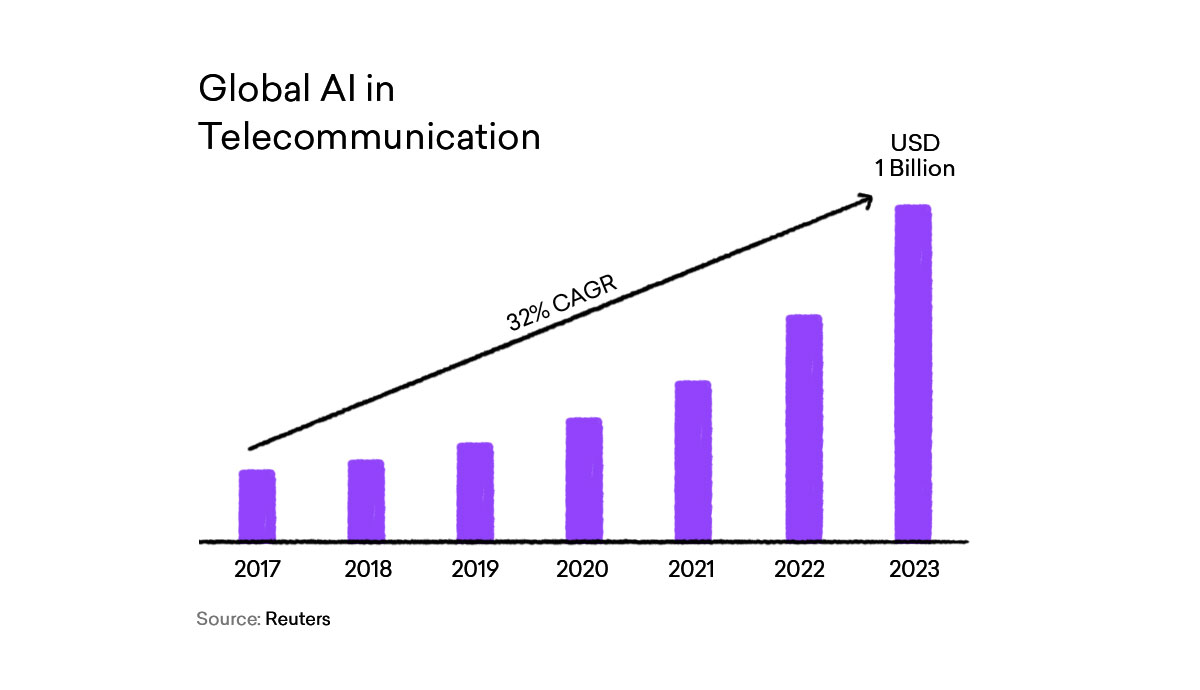
\includegraphics[width=1.0\textwidth]{imagenes/01_Introduccion/inversion_chatbots.jpg}
    \begin{center}
        Fuente: \url{https://es.aivo.co/blog/chatbots-in-telecom}
    \end{center}
    \caption{Estimación de la inversión en IA en el campo de las telecomunicaciones}
    \label{fig:inversion_chatbot}
\end{figure}

Para personas que están empezando a investigar para comprender los chatbots, se encuentran con la dificultad de la poca claridad de las revisiones bibliográficas existentes dado que adolecen de tres problemas notables (Referencia a PaPer state-of-the-art). En primer lugar, nos encontramos con el problema que aparece nada más empezar, y es la carencia de un esquema de clasificación de chatbots, dado que no se ha definido una clasificación global. La clasificación más extendida es la clasificación según el mecanismo de recuperación y de generación de respuestas, donde destacan los chatbots que hacen uso de bases de conocimientos estáticas, es decir, chatbots basados en reglas; y los chatbots que hacen uso de mecanismos de aprendizaje e inferencia adaptativos, es decir, los chatbots basados en inteligencia artificial. En segundo lugar, las revisiones están desactualizadas en el ámbito de la generación de respuestas dado el rápido avance de las técnicas computacionales. En tercer lugar, las revisiones no están muy centradas en la aplicación empresarial de los chatbots ni en su usabilidad, sino que más bien están centradas en el aspecto técnico.

La estructura de los chatbots ha ido evolucionando y extendiéndose. Originalmente la estructura de los chatbots era la descrita por Abdul-Kader y Woods, donde se podía reconocer tres componentes: interfaz, un clasificador y un graphmaster. Esta estructura está muy desactualizada a día de hoy, ya que en la estructura original la interfaz sólo tenía previstas entradas en forma de texto, pero hoy en día las entradas son de tipo multimedia, por lo que es necesario actualizar la interfaz a una interfaz multimedia, y añadir un nuevo componente a la estructura, encargado de manejar esas entradas multimedia y convertirlas en entradas de texto que se puedan manejar para generar respuestas; además dado el auge de los chatbots basado en generación, a día de hoy el componente del graphmaster no tiene sentido, dado que las respuestas se generan utilizando modelos preentrenados realizando inferencias en base a las entradas, por lo que tener un manejador para el almacenamiento de conocimiento deja de tener sentido, por lo tanto en la estructura el graphmaster debe ser actualizado por un modelo generador de respuestas. En base a todas estas actualizaciones sobre la estructura original de Abdul-Kader y Woods, obtenemos la estructura actual de los chatbots, que se muestra en la Figura \ref{fig:estructura_state_of_art}. Finalmente tenemos cuatro componentes: la interfaz, un procesador multimedia, un análisis de entrada multimodal y un generador de respuestas.

\begin{figure}[h]
    \centering
    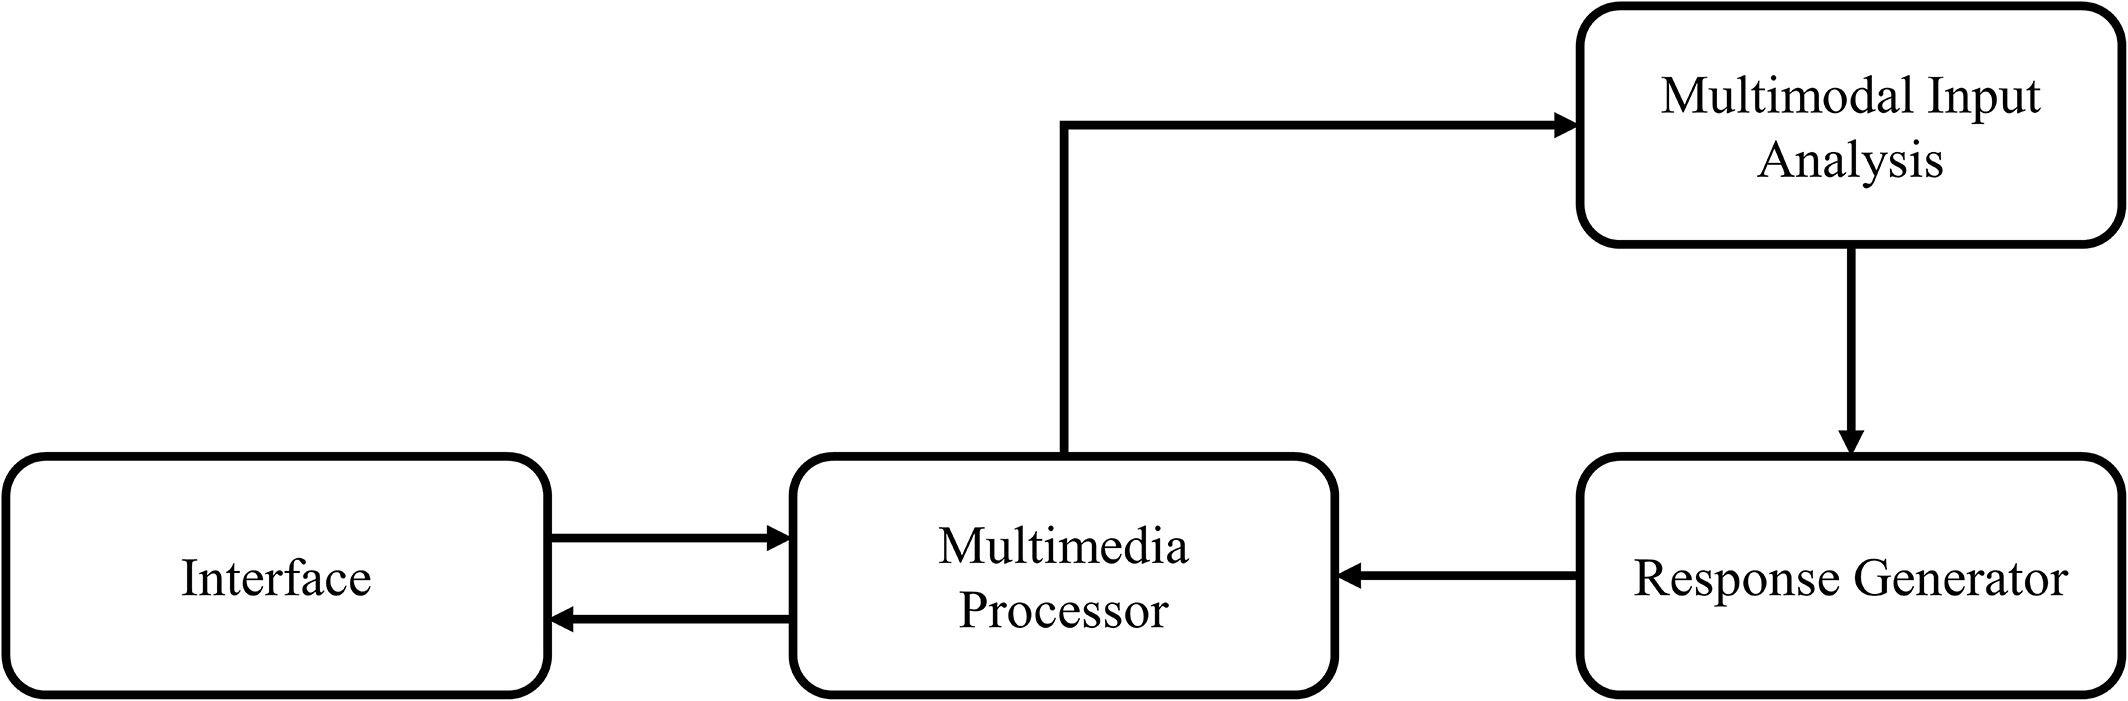
\includegraphics[width=0.8\textwidth]{imagenes/01_Introduccion/estructura_state_of_art.jpg}
    \begin{center}
        Fuente: A critical review of state-of-the-art chatbot designs and applications (Referencia a PaPer state-of-the-art)
    \end{center}
    \caption{Estructura de los chatbots actuales}
    \label{fig:estructura_state_of_art}
\end{figure}

Un componente que se muestra en la Figura \ref{fig:estructura_state_of_art} y que no se ha mencionado explícitamente cual es su labor es el análisis de entrada multimodal. Este análisis realiza un pretratamiento de los datos de entrada, hoy en día se intenta mejorar este componente con técnicas avanzadas de comprensión del lenguaje natural (NLU).

En el caso de los chatbots basados en la recuperación, el generador de respuestas desempeña el mismo papel que el graphmaster, ya que almacena y recupera las respuestas, mientras que en el caso de los chatbots basados en la generación, asigna la entrada normalizada transferida desde la unidad de pretratamiento de la entrada a la salida (Referencia a PaPer state-of-the-art).

Centrándonos en el componente del generador de respuestas, a día de hoy se utilizan distintas técnicas para implementar este componente. Las técnicas más destacadas son las siguientes:

\begin{itemize}
    \item \textbf{Template:} Esta técnica se compone de patrones y plantillas formando pares con ellos. Para generar las respuestas se busca el patrón que más concuerde con la entrada recibida, y una vez se haya elegido un patrón se devuelve la plantilla asociada al mismo. El lenguaje que más destaca en esta técnica es AIML \footnote{\url{http://www.aiml.foundation}}. La desventaja de tener que crear los archivos AIML se puede suplir mediante la extracción automática de conocimientos, reduciendo el trabajo manual. Los chatbots basados en plantillas son sencillos de crear por lo que tanto son una opción popular para chatbots a pequeña escala.
    \item \textbf{Corpus:} Son una buena técnica como alternativa a los template cuando se están contruyendo chatbots a gran escalas, debido a que con los templates al aumentar de escalas aumenta el número de patrones y trae consigo búsquedas más lentas lo que ralentiza la generación de respuestas. Existen dos tipos de chatbots basados en Corpus, un tipo de chatbots basados en corpu que no selecciona cuidadosamente el conocimiento y otro que si lo hace. El tipo que selecciona cuidadosamente el conocimiento se puede implementar mediante bases de datos ó mediante modelos de ontología, los modelos de ontología tienen una gestión más flexible del conocimiento que las bases de datos, la generación en este tipo de chatbots se realiza también con búsqueda pero esta vez en la estructuras descritas anteriormente. El tipo que no selecciona cuidadosamente el conocimiento transforma las palabras en vectores que representan los significados semánticos de las palabras en un espacio multidimensional, la generación en este tipo de chatbots se realiza mediante el cálculo de la distancia entre los pares de entrada del usuario y de consulta-respuesta, se empareja la consulta con la menor distancia y se selecciona su correspondiente respuesta como salida. Debido a la gran capacidad de gestión del conocimiento, varias aplicaciones que requieren un conocimiento formal del dominio utilizan chatbots basados en corpus (Referencia a PaPer state-of-the-art).
    \item \textbf{Intent:} Los chatbots basados en intenciones se utilizan ampliamente para los sistemas orientados a tareas que presentan diálogos de varios turnos (Referencia a PaPer state-of-the-art). En el caso de esta técnica es necesario añadir adicionalmente un componente de análisis de entrada multimodal (SLU), dentro de él se realiza un análisis semántico de las entradas, para este análisis se suelen utilizar técnicas avanzadas de NLU, además a partir del análisis semántico realiza una clasificación para saber a que intención pertenece la entrada mediante técnicas de aprendizaje automático. Dado que estos chatbots están orientados a tareas es necesario tener dentro de la generación de respuestas técnicas de DST para la identificación del estado del diálogo, y técnicas de DPO para el procesamiento del estado del diálogo; estas dos técnicas son necesarias para establecer la secuencia de los diálogos. Las bases de conocimiento de los generadores de respuestas en los chatbots basados en intenciones están compuestas principalmente de frases de entrenamiento, intenciones y respuestas. Para generar las respuestas se analiza semánticamente las entradas en el módulo SLU, posteriormente se utiliza el módulo DST para estimar el estado de los diálogos actuales y finalmente se utiliza el módulo DPO para determinar las acciones y respuestas. Este tipo de chatbots son utilizados por grandes empresas como puede ser Google con Dialogflow \footnote{\url{https://dialogflow.cloud.google.com}} (originalmente llamado Api.ai) o también existen alternativas de código abierto como puede ser Rasa \footnote{\url{https://rasa.com/}}.
    \item \textbf{Red neuronal recurrente (RNN):} Los chatbots creados con esta técnica dejarán de estar basados en la recuperación, como pasaba en las tres anteriores técnicas, sino que estarán basados en la generación, pero esto que quiere decir, en definitiva quiere decir que la generación de las respuestas no se realizará mediante búsquedas en alguna estructura y sustitución mediante pares consulta-respuesta. La generación de las respuestas se realiza mediante inferencias con modelo de redes neuronales recurrentes. Estos chatbots, a diferencia de los chatbots basados en intenciones, no están orientados a las tareas y esto deriva del problema que conllevan las redes neuronales, y no es otro que las redes convierten al chatbot en una caja negra, esto quiere decir que la respuesta del chatbot ante cierta entrada es incierta incluso para su creador, este inconveniente se convierte en una ventaja si orientamos a los chatbots al chat, dado que esta incertidumbre en la respuesta da una gran sensación de naturalidad y creatividad durante la conversación, por lo que son apropiados para actividad relacionadas con el entretenimiento y la salud mental. Estos chatbots se han visto muy potenciados en los últimos años debido al rápido desarrollo del aprendizaje profundo. Uno de los mayores hitos en el aprendizaje profundo ha sido la creación de GPT-3 \footnote{\url{https://openai.com/blog/openai-api}}, el cuál es un nuevo modelo de inteligencia artificial que permite generar lenguaje escrito creado por la empresa OpenAI. Como se ha mencionado anteriormente ya no se realiza recuperación para la generación de respuestas, por lo tanto las bases de conocimiento de los chatbots basados en RNN estarán compuestas de los conjuntos de datos de entrenamiento. El resultado de los chatbots basados en la generación depende de la especificación del modelo, los conjuntos de datos de entrenamiento, el proceso de entrenamiento y la entrada del usuario (Referencia a PaPer state-of-the-art).
    \item \textbf{Aprendizaje por refuerzo (RL):} Este tipo de chatbots suelen estar basados en la recuperación y utilizan plenamente el contexto de entrada para la búsqueda de respuestas óptimas (Referencia a PaPer state-of-the-art). Dado que se basan en la recuperación, en sus bases de conocimientos hay pares de consulta-respuesta predefinidos. El método RL se basa principalmente en el proceso de decisión de Markov. Al igual que pasaba en los chatbots basados en templates, en los chatbots basados en RL se utlizan representaciones vectoriales, en concreto el estado del chatbot es una representación vectorial de un turno de conversación. Este vector puede contener la respuesta derivada de la entrada ó adicionalmente puede contener el acto de diálogo, el sentimiento del usuario y el enunciado genérico del usuario. El contexto de la comunicación forma una secuencia de estados. Aunque es una técnica basada en la recuperación, esta recuperación es distinta a la descrita en las anteriores técnicas, en el caso de esta técnica se utiliza una política para encontrar la respuesta adecuada, esta política debe ser bien entrenada para lo que son necesarios diálogos predefinidos. Este tipo de chatbots se pueden utilizar para secciones de "Preguntas frecuentes".
    \item \textbf{Enfoques híbridos:} El intento de combinar varias técnicas para suplir las desventajas de ambas con las ventajas de cada técnica es algo que se ha intentado en una multitud de ámbitos, y este no iba a ser menos. En el paper (Referencia a PaPer state-of-the-art) se hace referencia a una serie de propuestas de diferentes investigadores. Una de ellas puede ser la propuesta por Li Wu  y Wu Wu propusieron un marco de correspondencia secuencial basado en una RNN. El marco considera las relaciones entre los enunciados anteriores y las respuestas candidatas y selecciona las respuestas óptimas para el contexto.
\end{itemize}

Si nos fijamos en la técnica utilizada para crear el chatbot podemos obtener una buena clasificación de los mismos.

Una vez estudiada la estructura actual de los chatbots. A continuación voy a exponer algunas de las posibles aplicaciones que pueden tener los distintos chatbots.

La primera aplicación y puede que la más usada por la gente en general es la atención al cliente para el comercio electrónico. Dado el gran crecimiento de sector, se ha producido un elevado aumento de la carga de trabajo. Como se ha indicado anteriormente, por ejemplo en el caso de los chatbots basados en intenciones, los chatbots son capaces de reducir la carga de trabajo y consecuentemente también reduce los costes humanos. La calidad del servicio proporcioando por estos chatbots está en continua mejora debido a la dificultad de manejar peticiones muy complejas por parte del usuario y otros problemas como el amplio dominio necesario para contestar de forma correcta durante toda la conversación y no sólo para contestar si no también para realizar un servicio agradable para el usuario.

La siguiente aplicación a exponer también está muy extendida y es usada asiduamente por multitud de personas. Los chatbots de asistencia personal pueden utilizarse para aumentar la eficiencia del trabajo ó para gestionar la vida cotidiana del usuario. Un posible ejemplo podría ser Siri \footnote{\url{https://www.apple.com/es/siri}}, que es un chatbot incorporado en todos los dispositivos iPhone.

Otra posible aplicación de los chatbots es la asistencia sanitaria. Este clase de chatbots actuan como asistentes médicos para el diagnóstico de enfermedades. La comprensión de los síntomas del paciente es primordial en el proceso de detección de la enfermedad, y una de las principales funciones de estos chatbots es recoger suficiente información de los pacientes (Referencia a PaPer state-of-the-art). Aunque en los aspectos médicos la última palabra la tiene un profesional humano, los chatbots puede realizar diagnósticos previos rápidamente dada su inmenso conocimiento al que se puede acceder en un instante, cosa que no sucede con los humanos lo que ralentiza el diagnóstico. Esta enorme base de conocimiento es muy importante en la medicina debido al vasto dominio de este campo.

Y como última aplicación a exponer tenemos los agentes conversacionales pedagógicos. Estos chatbots están diseñados para ayudar al aprendizaje. Dado que la función principal de los chatbots es comunicarse con los usuarios, el aprendizaje de idiomas ha sido una de las principales vías perseguidas (Referencia a PaPer state-of-the-art), ya que el aprendizaje de idiomas está a la orden del día de todo el mundo. Estos chatbots son útiles para enseñar a usuarios mediante conocimientos de expertos, sin que sea necesario una ingente cantidad de expertos para enseñar, ya que esta cantidad de expertos en ciertos campos y lugares no está disponible.

En todas estas aplicaciones existe el problema de la seguridad de los datos necesarios por el chatbot, este aspecto está muy presente en los últimos años debido a los múltiples casos publicados sobre falta de seguridad con los datos de los usuarios. De cara al futuro se pretende que aumente la seguridad de estos datos.

LLegados a este punto en el que ya hemos analizado el estado actual de los chatbots, sólo nos queda analizar cuál es la dirección de las futuras investigaciones en este sector. Estas investigaciones estarán centradas en paliar las deficiencias actuales y en mejorar aún más las capacidades actuales.

Uno de los principales problemas de los chatbots es la ingente cantidad de datos que necesitan para empezar a funcionar. Actualmente este conocimiento es almacenado en estructura de distinto tipo, sin tener un esquema unificado. Esta variedad de bases de conocimiento distintas dificulta la creación de nuevos chatbots al no poder reutilizar datos utilizados en chatbots anteriores. Una posible futura mejora sería la estandarización de la gestión del conocimientos para poder realizar esta transferencia de datos entre chatbots de forma eficiente.

Un aspecto analizado anteriormente es la generación de las respuestas, este aspecto aunque ha sufrido un gran desarrollo en los últimos años, todavía no ha llegado a alcanzar su máximo nivel, esto se puede comprobar simplemente con ver, tal y como indica el paper (Referencia a PaPer state-of-the-art), que todavía nadie a ganado el premio de oro del Premio Loebner, el concurso de pruebas Turing más famoso en el ámbito de los chatbots. Las futuras investigaciones están orientadas a la mejora de las técnicas de aprendizaje profundo. Estas técnicas son entre otras las redes generativas adversativas (GAN), este tipo de redes está muy extendido en el mundo de la visión por computador pero todavía no se ha llegado a conseguir un integración de esta técnica en el mundo de los chatbots.

Un aspecto de los chatbots que todavía tiene mucho potencial por explotar es sin duda la interfaz. Hasta ahora sólo hemos indicado que se están utilizando interfaces multimodal. Pero no se está sacando todo el partido a este tipo de interfaces, dado que actualmente sólo se realiza un conversión de todo tipo de entradas a una entrada en formato de texto. Pero las entradas multimodal contienen información adicional a la que se extrae hoy en día, como puede ser el lenguaje no verbal durante una conversación por voz. Este lenguaje no verbal proporciona mucha información que puede ayudar a la generación de respuesta y a tener un mejor contexto de la conversación. Para que toda esta información no se desperdicie se debe avanzar en la investigación para la extracción de esta información. Otro aspecto de la interfaz donde es necesaria la investigación es la devolución de la respuesta a través de la interfaz, ya que hasta ahora estábamos hablando de como se debía mejorar la entrada de información en la interfaz. La devolución de esta información se puede realizar de muchas manera, escrita, por voz, etc. Lo verdaderamente importante en la devolución de la respuesta es que el usuario perciba esa respuesta con facilidad, con una buena estética que atraiga la atención del mismo. Una de las líneas de futuras investigaciones son los avatares 3D, es decir, la respuesta es devuelta por voz pero lleva añadida la gesticulación de un avatar 3D.

Una dirección en la que se pueden realizar futuras investigaciones son las aplicaciones del chatbot. Dado el auge del internet de las cosas (IoT) hoy en día hay todo un campo donde integrar los chatbots para mejorar el servicio a los usuario, como pueden ser los coches inteligentes, los hogares inteligentes, y muchos más.

Por último, tal y como se ha indicado anteriormente, uno de los grandes problemas actualmente de lo chatbots es la falta de seguridad con los datos, este es un aspecto crucial en todas las futuras investigaciones.






\section{Licencia}


